\section{MTConnect in OPC UA}

\begin{quote}
    \color{red}
    TODO: This section will need to be rewritten with the new activity and data flow models and the factories to create the information models.
\end{quote}

\subsection{Base Information}

It is expected that MTConnect and OPC UA will continue to evolve their respective standards, in particular as the MTConnect defined information model is revised an OPC UA Client may desire to know the version of the MTConnect model implement by a given server. The information model will always be backwards compatible.

MTConnect defines a Probe request, which is just mapped to an OPC UA Browse. The Probe request returns the devices that are defined in an agent. In OPC UA, a client can at any time browse the address space, and return the detailed structure of the address space, this includes all relationships between devices, their defined types and data types. An OPC UA Client can also subscribe for a \texttt{ModelChangeEvents} changes and \texttt{SemanticChangeEvents} which allow the client to be notified if the address space is modified. \texttt{ModelChangeEvent} are generated by server whenever a new node or reference is added to a server. The Node may be a new type definition, change to a type definition or a new instance node. \texttt{SemanticChangeEvents} are generated by a server when some aspect of an instance of a node type is change and the change would result in a change that a client should be aware of. An example of a \texttt{SemanticChangeEvent} would be for a change in the engineering Unit assigned to a node.

MTConnect defines a Sample Request command to obtain information from the device. This command can be mapped to an OPC UA read or subscription service. The read service will return the latest value of the requested item. This is appropriate for obtaining the most recent value of a variable. The Subscription service is described the next paragraph. In some cases Historical data access may be required. This allows a client to obtain older values for a device, based on time ranges or other criteria. This feature can be used by a server to allow addition data to be available and could be used to enhance MTConnect Sample Request for cases where more than just the current value is required.

MTConnect describes a Streaming command, which matches to the OPC UA subscription service. This service would allow a client to obtain a steady stream of values associated with a device. The subscription service supports filtering, based on data changes or even aggregates, where an aggregate is a minimum, maximum, average, time in state or any of a long list of aggregates. For a complete list of OPC defined aggregates see \cite{UAPart11}. It would also allow the return of any OPC Events associated with the device. An OPC Event in MTConnect terms would be a transition of a Condition. Subscription data includes message information that allows a client to determine if a packet was missed or is out of order. The client can request a replay of any missed information or re-sequence the packets. Also included is a keep-alive heart beat that allows for rapid determination of and recovery from communication failures. This functionality is used to ensure the MTConnect Streaming functionality is matched.

MTConnect error codes will be mapped to OPC UA error codes where appropriate. The OPC UA server has a multilevel error reporting capability. A Service can include  	 information, as well as the individual data items that are being reported as part of the service.

As discussed in the overview of OPC UA, all companion specifications usually define a \texttt{Namespace}. For this companion specification all \texttt{Type\-Definitions} and \texttt{Browse\-Names} defined by this specification are qualified by the MTConnect \texttt{Namespace} \\
\texttt{("urn:mtconnect.com:MTConnectDevices:1.2")} unless stated otherwise.

The description associated with MTConnect items is always mapped to the Description attribute available in OPC UA.

\FloatBarrier
\subsection{Additional Subscription Information}

A \texttt{DataChange} Subscription can be created with the following steps:

\begin{itemize}
\item Browse the Address Space and read the NodeIds for the DataItems of interest;
\item Create a Subscription;
\item Create a MonitoredItem for each DataItem of interest;
\end{itemize}

As an alternative to browsing the address space, a browse path from a starting node can be created using the type definitions and the \texttt{TranslateBrowsePathsToNodeIds} service can be called to obtain the actual \texttt{NodeIds}. Figure \ref{fig:browse_path_ex} provides an example of a data item that is for a know type. The illustrated path is the same for any instance of a boiler object.

\begin{figure}[h]
  \centering
  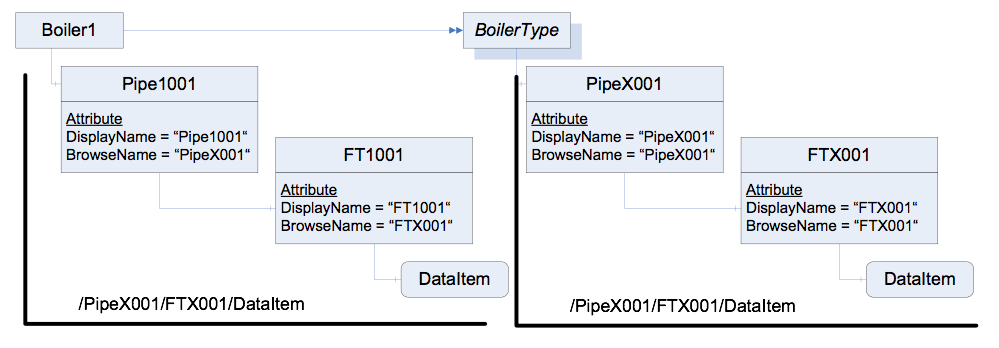
\includegraphics[width=1.0\textwidth]{diagrams/BrowsePathEx.png}
  \caption{Browse Path Example}
  \label{fig:browse_path_ex}
\end{figure}

Each Notification has the current value for a \texttt{DataItem}, the \texttt{Timestamp} and \texttt{Status\-Code}.

The \texttt{MonitoredItem} allows the Client to specify a different SamplingInterval and \texttt{QueueSize} for each \texttt{DataItem}. The \texttt{MinimumSamplingInterval} attribute for each \texttt{DataItem} specifies the fastest supported \texttt{SamplingInterval}. The \texttt{Publishing\-Interval} for a Subscription controls how frequently Notifications are returned to the Client. If this value is longer than \texttt{Sampling\-Interval} then the Server will buffer changes and return multiple Notifications in one message. 

An OPC \texttt{Event} Subscription can be created with the following steps: 

\begin{itemize}
\item Browse the Address Space and read the \texttt{NodeIds} for the Devices or \texttt{Components} of interest;
\item Create a Subscription;
    \begin{itemize}
    \item Create a \texttt{MonitoredItem} for each Device or Component of interest;
    \item Select the fields to return for each event, where the complete list of available fields is defined as part of the OPC UA \texttt{EventType} definition;
    \item Specify additional filter criteria for the events to return; 
    \end{itemize}
\end{itemize}

Events in OPC UA propagate up the \texttt{HasNotifier} hierarchy. This means subscribing to a parent Node in a hierarchy (i.e. an MTConnect Device) will request events for all Components under that Node. If a Client wants to receive all events for all devices it can subscribe to the Server node.
Each Condition Event is a snapshot of the \texttt{MTConditionType} Object. The Client must select the fields from the Condition that it wishes to receive in the update by specifying the \texttt{BrowsePath} (a sequence of \texttt{BrowseNames}). 

\begin{quote}
    \color{red}
    TODO: Need to provide model of event and condition management in MTConnect. Activity Models will be added here..
\end{quote}

\clearpage
